
\chapter{Problem definition}

This chapter describes the process of identifying the main needs of the stakeholders and defining the scope of the project. \textbf{TODO}

\section{Background}

Describe current situation....

\section{Requirements gathering}

In this section we aim to elicit the needs of the users and structure them into high-level system features that will later be designed and implemented.

\subsection{Stakeholders}

Stakeholders are the people that are have some kind interest in the project. They are the ones that will be affected by the project and thus they are the people that will be the source for the characteristics of the system we have to build. We identified the following as the main stakeholders of the project:  

\begin{itemize}
\item Scientists - people that develop algorithms and approaches for user modeling and analysis and allow other scientits and users to access them.
\item ImReal - system that want to use the services provided by the scientists and has its own requirements
\item RDFGears - provide the workflow engine and want to reuse some of the things.
\end{itemize}

\subsection{Interviews}

Once we had identified the stakeholders of the project we started to think how to extract the requirements from them. Literature suggest a wide variety of possible approaches []. However, there is one technique that proves to be really effective and it is the semi structured interviews \cite{Dieste}. In order to perform it we prepared some important questions that we wanted to know and then we did discussions \textbf{TODO}

\subsection{Identified features}

We analysed carefully all the raw information that we gather from the interviews and we identified several high-level features. We presented them to the stakeholders and after some discussions we ended up with the following final features that the system should provide: 

\begin{itemize}

\item \textbf{Multiuser support and Access control}
The system should allow access to multiple users simultaneously. It should also provide access control mechanism that deals with the following issues:\\
User types and authorization - What anonymous users are able to do and what registered user are able to do?\\
Information privacy - Users should be able to protect private or sensitive information.\\
Sharing and collaboration - How can users work together and reuse each other's work?

\item \textbf{Plug-in environment}
The system should enable scientists to extend it by plugging in custom logic such as RDFGears functions and other functional components. Users should be able to manage(add/update/remove) this custom logic runtime(without restarting the system). This process should not affect the work of other users.
 
\item \textbf{Scheduling}
The system should provide functionality that enables users to schedule and monitor the execution of workflows. 

\textbf{TODO}:
What should be made clear is what events are available in  scheduling. For example, configure to run on a specified date/time/interval. Or based on the completion of another component or workflow. Or based on the outcome (true/false) of a component, such that you can trigger it based on whether or not you found something in a crawl. 

\item \textbf{Universal data storage} 

Many of the workflows need to store various types of data(e.g. intermediate and final results). Therefore, the system should provide a mechanism that enables storage and retrieval of information in arbitrary data formats.

 
\item \textbf{Integration with Hadoop}
The amounts of information that have to be processed in the system can sometimes be huge. It is critical that this information is processed efficiently and Hadoop is often the solution for that. Therefore, the system should provide functionality that enables easy integration with Hadoop.

\end{itemize}

\section{Feature prioritization}

Having already defined the requirements we have to define the order in which we are going to design and implement them. Requirements(features) prioritization is the process of determining the order in which candidate requirements or features of a software product should be implemented. The criteria to order the requirements can vary a lot, for example one can consider the requirements' importance, value, cost, risks or views of stakeholders etc. Scientists and other systems(ImReal) that depend on U-Sem already need the functionality and thus we are mainly concentrated to deliver the most essential functionality as early as possible. Having this in mind, the criteria we choose for the prioritization is the value(importance) of each functionality as well as the time required for implementation(cost).

Requirements prioritization is a relatively old research topic and there are numerous approaches that are available \cite{Moisiadis}. The most popular include Quality Function Deployment (QFD) the Analytical Hierarchy Process(AHP), the cost-value approach proposed by Karlsson, Wiegers' method, as well as a variety of industrial practices such as team voting, etc. However, literature also suggests that there is no perfect solution for this problem and the applicability of each approach depends heavily on the particular situation it is used.

For our project, we choose the Karlsson's Cost-Value approach that makes use of the analytic hierarchy process \cite{Karlsson}. This decision was based on several factors. Firstly, it uses the exact criteria that we are interested in(value and cost). Secondly, it is especially suitable for prioritizing a small number of requirements\cite{Karlsson}, which is our case. And last but not least, it is a proven and widely used \cite{Karlsson2}.


\subsection{Requirements prioritization using the Cost-Value Approach}

In this section we will describe step by step the process of prioritizing requirements using the Cost-Value approach. The process consists of three distinct steps. The following sub-sections will address these steps.

\subsubsection{Value assessment}

In the Requirements gathering section we identified 5 high-level requirements(features) that cover the main functionality of the system. In this step we are using the AHP's pairwise comparison method in order to assess the relative value of the candidate requirements. We asked a group of four experienced project members to represent customers views. We instructed them on the process and asked them to perform  pairwise comparisons of the candidate requirements based on their value(importance). For the comparison criteria we used the one defined in \cite{}. Fig.. Apendix 1 shows the form that they were asked to fill.

We let the participants to work alone, defining their own pace. We also allowed them to choose the order of the pair's comparison. Discussions were also allowed. When all participant finished the pairwise comparison, we started to calculated the value distribution. However, first we calculated the the consistency indices of the pairwise comparisons. According to \cite{AHP}
 values lower than 0.10 are considered acceptable and according to \cite{Karlsson} values around .12 are commonly achieved in the industry and can also be considered acceptable. The calculation showed that two of the participants has indeces higher than .23 which indicates serious inconsistencies. Therefore, we asked them to revise their answers and the results were around 0.12 \textbf{TODO}
 
 \begin{table}[h!]
  \begin{center}
    \begin{tabular}{| l | l | l | l | l |}
    \hline
    & Stakeholder 1 & Stakeholder 2 & Stakeholder 3 & Stakeholder 4 \\	 \hline
    Consistency ratio & 0.04 & 0.23 & 0.13 & 0.26 \\
    \hline
    \end{tabular}
  \end{center}
  \caption{The initial consistency ratios for each of the stakeholders.}
\end{table}


 \begin{table}[h!]
  \begin{center}
    \begin{tabular}{| l | l | l | l | l |}
    \hline
    & Stakeholder 1 & Stakeholder 2 & Stakeholder 3 & Stakeholder 4 \\	 \hline
    Consistency ratio & 0.04 & 0.12 & 0.13 & 0.11 \\
    \hline
    \end{tabular}
  \end{center}
  \caption{Consistency ratios for each of the stakeholders after refinement.}
\end{table}

Once we had achieved satisfying results we calculated the distributions. We outlined the candidate requirements in a diagram and presented the results to the project members. Each requirement's determined value is relative and based on a ratio scale. Therefore, a requirement whose value is calculated as 0.20 is twice as valuable as a requirement with a value of 0.10. Additionally, the sum of the values for all requirements equals 1. This means that a requirement with a value of 0.10 provides 10 percent of the value of all the requirements. You can see that the "plug-in environment" requirements is the most valuable. It is followed by the "data-store" and "Access control". At the bottom, providing considerably less value, are the "scheduling" and "hadoop" requirements.

\begin{figure}[h!]
  \centering
      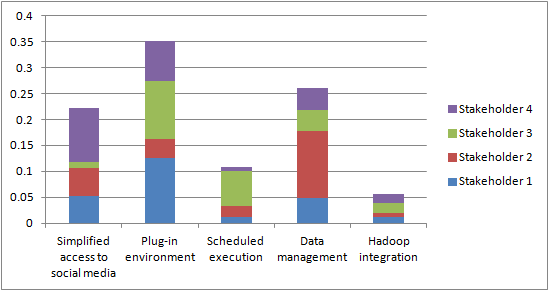
\includegraphics{requirements/value_diagram.png}
  \caption{The value distribution of the 5 requirements in the U-Sem project.}
\end{figure}

\subsubsection{Cost assessment}

Value on its own is not enough to estimate the priority of the requirements. The problem is that a requirement with high value may also be costly to implement and also take a lot of time. Our aim is to provide the most value as quick as possible. Thus, requirements that provide a bit less value but on the other hand are easy and quicker to implement might be the better choice. In this step, we measure the distribution of cost between the requirements. In order to do that, we asked the software engineer responsible to build the system to perform AHP's pairwise comparison to estimate the cost of implementing each of the candidate requirements. The process absolutely the same as the one described in the previous section. However, this time the requirements are compared based on their cost rather than their value.

Once the comparison was finished, we measured the consistency index of the answers. The result was \textbf{0.029} which is completely acceptable and there was no need for further refinement.

Finally, we used the AHP technique to calculate the cost distribution of the requirements. We outlined the results in a digram FIG. Again, the determined values are relative and based on a ratio scale. 

\begin{figure}[h!]
  \centering
  	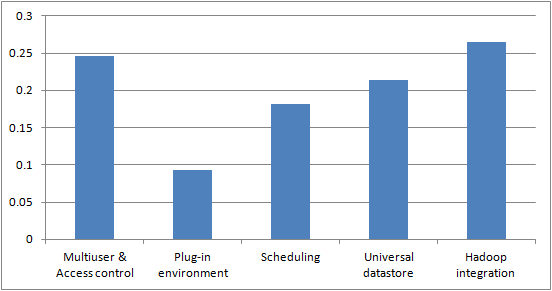
\includegraphics{requirements/cost_diagram.png}
  \caption{The cost distribution of the 5 requirements in the U-Sem project.}
\end{figure}
 

\subsubsection{Cost-Value analysis}

Once we have the value and cost value distribution of the requirements we can establish the order in which to implement the requirements. The decision is based on the value/cost ratio of each requirement. Figure[] shows the results. As you can see, the the plug-in environment is the definite winner and the hadoop integration provides very little benefit compared to the cost to implement it.

\begin{figure}[h!]
  \centering
      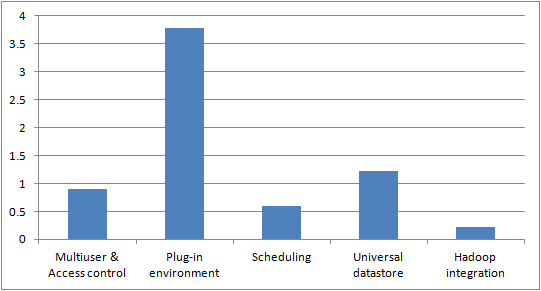
\includegraphics{requirements/value_cost_diagram.png}
  \caption{This diagram shows the comparison of the value/cost ratio of the requirements.}
\end{figure}

\subsubsection{Discussion}

Our observations about the stakeholders which were asked to perform the pairwise comparisons found the method intuitive and easy to understand. However, they also found performing the pairwise comparison to be a bit tedious. They sometimes got distracted and gave inconsistent results which was indicated by the consistency check. However, this was easily fixed by revising the answers and we reached a level of consistency that is considered acceptable.

Another disadvantage of this approach that affected our work is the fact that the method takes no account of interdependencies between requirements. However, this issue did not affect the project significantly because the project high-level features are loosely coupled and the only one that required some attentions was the "access control". \textbf{TODO}



\begin{thebibliography}{99}

\bibitem{Dieste}
Oscar Dieste, Natalia Juristo, and Forrest Shull, Understanding the Customer: What Do We Know about Requirements Elicitation?
\bibitem{Karlsson}
Karlsson, J., Ryan, K. (1997). A Cost-Value Approach for Prioritizing Requirements, IEEE Software September/October 1997, 67-74.

\bibitem{Karlsson2}
J Karlsson, C Wohlin, B Regnell - Information and Software Technology, 1998 - Elsevier

\bibitem{Moisiadis}
Frank Moisiadis, THE FUNDAMENTALS OF PRIORITISING REQUIREMENTS

\end{thebibliography}